\documentclass[preprint,aps]{revtex4}
\usepackage{graphicx}

\newcommand{\ax}{{\bf a}_1}
\newcommand{\ay}{{\bf a}_2}
\newcommand{\Ax}{{\bf A}_1}
\newcommand{\Ay}{{\bf A}_2}

\begin{document}
\title{Packing Squares in a Torus}

\author{D. Blair}
\email[]{dwblair@physics.umass.edu}
\affiliation{Department of Physics,
University of Massachusetts,
Amherst, MA 01003-3720, USA}

\author{J. Machta}
\email[]{machta@physics.umass.edu}
\affiliation{Department of Physics,
University of Massachusetts,
Amherst, MA 01003-3720, USA}
\affiliation{Santa Fe Institute, 1399 Hyde Park Rd, Santa Fe, NM 87501, USA}

\author{C. Santangelo}
\email[]{santangelo@physics.umass.edu}
\affiliation{Department of Physics,
University of Massachusetts,
Amherst, MA 01003-3720, USA}

\begin{abstract}
The densest packings of $N$ unit squares in a torus are studied using analytical methods as well as simulated annealing.  A rich array of dense packing solutions are found: density one packings when $N$ is the sum of two square integers; a family of ``gapped bricklayer'' Bravais lattice
 solutions with density $N/(N+1)$; and some surprising non-Bravais lattice configurations, including lattices of holes as well as a configuration for $N=23$ in which not all squares share the same orientation.  The entropy of some of these configurations and the frequency and orientation of density one solutions as $N \rightarrow \infty$ are discussed.

\end{abstract} 
\maketitle
\input{squares_torus_intro.tex}
\input{square_torus_analytics.tex}
%\input{squares_torus_proofs.tex}
\section{Numerical Methods}
\label{sec:numerical}

%\subsection{New Mat}
%\subsection{Overview}
%Rintoul and Torquato, ``Computer Simulations of dense hard-sphere systems'' \cite{Rintoul1996a}
For all $N \leq 27$ squares on the flat torus, we searched for densest packings of $N$ squares on the torus via Monte Carlo simulations in the NPT ensemble.  Our approach was to perform simulated annealing (SA), in which the system was taken from an initial, low-pressure, easy-to-equilibrate state to a final, high-pressure state via an annealing schedule consisting of a series of steps in inverse pressure.  Between each pressure increase, a Metropolis algorithm appropriate to the hard square NPT ensemble was used to equilibrate the system.  Although SA quickly falls out of equilibrium at higher pressures as the energy landscape becomes rough, it appears to be an an effective algorithm for finding ground states of the system.  

%Population annealing: \cite{Hukushima2003}

%We used two related approaches to finding ground states: simulated annealing (SA) [REF??] and population annealing (PA) \cite{Machta2010a}.  SA and PA are Monte Carlo techniques that can been used to find ground states of systems with rough energy landscapes and multiple metastable states.  In both SA and PA, the system is taken from an initial,  low-pressure, easy-to-equilibrate state to a final, higher-pressure state via a series of steps in inverse pressure -- an annealing schedule. Between these pressure increases, an equilibration procedure -- in our case, a Metropolis algorithm appropriate to a hard-particle NPT ensemble, described in Section [??] -- is used in an attempt to equilibrate the system.  In SA, the system quickly falls out of equilibrium at higher pressures as the energy landscape becomes rough; nevertheless, SA remains an effective algorithm for finding ground states of a system, and is used widely in [examples].  PA [Machta and Ellis REF, Machta REF] is a way of keeping the system close to equilibrium by adding an additional step to the annealing procedure.  In PA, a collection of identical systems, or replicas, are simulated in parallel.  As in SA, all replicas are taken through a compression schedule; but in PA, after each compression, the collection of replicas is 'resampled':  some replicas are copied, and others are destroyed, in order to achieve a distribution of replica volumes that approximates the expected equilibrium Boltzman distribution at the current pressure.  Details of this procedure are described below in section [??].  We simulated several replicas using both SA and PA, and took the highest density configuration for a given $N$ found using either procedure as our best candidate for the ground state of the system.

%\subsection{Algorithm Details}
The equilibration procedure we used in our simulated annealing algorithm was a Metropolis procedure consisting of three types of Monte Carlo moves:  translations and rotations of individual squares, and changes in the volume of the entire system.  At each step of the equilibration procedure, a square is selected at random, and then one of the three types of moves is selected at random, with probabilities .495, .495, and .01 for translation, rotation, and volume change, respectively.  Once a square and a move type is selected, the move is attempted.  If the move results in any overlaps among the $N$ squares, the move is rejected.  If it does not, then for translations or rotations, the move is accepted; for volume change $dV$, the move is accepted with probability $p_{acc}=\min[1,\exp(-\beta P dV)]$.  In practice, rather than changing the volume of the entire system, the periodic box in the simulations was kept at a constant size, and the sizes of the individual squares were all rescaled, in order to achieve the desired new volume. The equilibration procedure consists of $s$ such Monte Carlo steps; in our simluations, $s$ was typically between 200 and 400 steps.  

We repeated this simulation 1,000 times, and reported the highest density found among these runs.  In order to determine the highest-density packing for $N$ that did not correspond to a perfect square or a sum of squares, more extensive runs were conducted -- as long as 72 hours on a 2GHz processor in some cases.  The fact that significantly different initial configurations and different initial random seeds generated the same final, high-density configurations signalled that we had found a good candidate for a densest packing of the system.  For all simulations, the pressure was initially set to $\beta P=.01$ and was increased via constant steps in inverse pressure until a maximum pressure of $\beta P_{max}=3000$ was reached. (During subsequent explorations of the phase behavior of the system, this pressure was later deemed excessive; but nevertheless produced reasonable results for the purposes of determing the ground state of the system.) All simulations were begun at an initial areal density $\rho$ of 0.1 with a square array of unit squares. Before each equilibration procedure began, a trial run was conducted in which the maximum value of translations, rotations, and volume changes were independently optimized in order to achieve an acceptance ratio for each of $0.4$. 

The majority of the computational work during the equilibration procedure consisted in checking for square overlaps.  For this, we relied on a fast algorithm for detecting polygon overlaps by Alan Murta [REF], and an associated Python wrapper by Joerg Raedler [REF].
%the General Polygon Clipping Library by Alan Murta (http://www.cs.man.ac.uk/~toby/alan/software/), and the Python wrapper written for this by Joerg Raedler (http://www.j-raedler.de/projects/polygon/).

Configurations were visualized using the VPython library (http://vpython.org/).


%\subsubsection{Population Annealing}

%As described above, SA consisted in taking a system (or several replicas of a system) through an annealing schedule of constant steps in inverse pressure, followed by $s$ equilibration moves after each pressure increase, until reaching a pressure at which the density appears to plateau. PA also involvs constant steps in inverse pressure, but after each pressure increase from the current pressure $P$ to the new pressure $P'$, the collection of $R$ replicas is 'resampled' so that the number of copies of a replica $j$ in the population reflect its expected equilibrium weight in the population, $w_j=\exp[-(P'-P)V_j]$. Copies of each replica $j$ are thus made in order to approximate the expected number of copies of replica $j$ in the population, 
%\begin{equation}
%p_j=\exp[-(P'-P)V_j]/Q,
%\end{equation}

%where 

%\begin{equation}
%Q=\Sigma_{j=1}^R exp[-(P'-P)V_j]/R
%\end{equation}

%Thus the appropriate number of copies of each replica can be generated by sampling from the multinomial distribution using $R$ trials [REF].  This is accomplished via a simple algorithm [REF, wikipedia, Multinomial Distribution ]: 


%\begin{enumerate}
%\item Initialize: $Q$
%\item For $i$ in range $(0,R)$:
%\begin{enumerate}
%\item $p_i=exp[-(P'-P)V_i]$
%\item $Q=Q+p_j$
%\end{enumerate}
%\item For $i$ in range $(0,R)$:
%\begin{enumerate}
%\item $p_i=p_i/Q$
%\item $X_i=\mathcal{R}(0,1)$
%\end{enumerate}
%\item Sort $X$ in ascending order
%\item Initialize: $p_{sum}$, TempReplicas, and $C$
%\item For $i$ in range $R$:
%\begin{enumerate}
%\item $p_{sum}=p_{sum}+p_i$
%\begin{enumerate}
%\item While ($C<R$) and ($p_{sum} \ge X_i$) do:
%\begin{enumerate}
%\item $C=C+1$
%\item TempReplicas[count]=Replica[i]
%\end{enumerate}
%\end{enumerate}
%\end{enumerate}
%\item For $i$ in range $(0,R)$:
%\begin{enumerate}
%\item Replica[i]=TempReplica[i]
%\end{enumerate}
%\end{enumerate}

%Where $\mathcal{R}(0,1)$ is a random number between $0$ and $1$.

%$\underset{x}{\operatorname{argmax}} $

% 1. Sort the replicas in descending order by volume; 2. For i in range(0,R):pick a random number $X$ from (0,1); choose replica $j= arg min (j'=1 to k) (\Sigma p_i >= X)$ to replace replica $i$ with a copy of replica $j$.  


%\begin{pseudocode}{Repopulate}
%\FOR i \GETS 0 \TO R \DO
%test of this line\\
%test of this line
%\end{pseudocode}

%\subsection{Results}

%A detailed analysis of the configurations found via simulation is found in Section~\ref{sec:analytics}.  For both SA and PA, our Monte Carlo simulations yielded a collection of replicas of varying densities at each pressure.  As the simulations for each $N$ progressed, we selected the highest-density configuration at each pressure using SA or PA as the candidate ground state for that $N$; the highest density reached in this manner was our best candidate for a ground state for $N$.  In Figure [?], we plot density $\rho$ vs. pressure $P$ for $N=12$ using both SA and PA.  This plot highlights a general trend:  for all values of $N$, the highest density among the PA replicas initially increased faster than that among the SA replicas at a given pressure.  In some cases (exemplified in Figure [?]), SA eventually overtook PA in density, finding a higher density configuration than any reached by PA; in others, PA found the highest-density configuration.  Figure [?] shows a simulation run for which the densities of both SA and PA had plateaued at nearly identical densities, and the associated configurations of each highest-density replica.  [SOME WORDS HERE RE: HOW EXTENSIVE OUR SIMULATIONS WERE IN CPU HOURS, HOW MUCH OF PARAMETER SPACE WE EXPLORED, AND HOUR HIGH CONFIDENCE THAT WE HAVE FOUND THE GROUND STATES FOR $N \leq 27$.  For some configurations (mentioned in Section~\ref{sec:analytics}), the ground state quickly approached density = 1 (for $N$ equal to a perfect square, e.g. 4, 16; or for $N$ equal to a sum-of-squares, e.g. 7, 10), and were provably optimal packings for that $N$; for other configurations, we are constrained merely to report our highest-density configuration as the best candidate thus far for a ground state for that $N$. In particular, the densities for $N=12,21,23$ consistently plateaued at their reported final values across several runs, and resulted in configurations that display obvious symmetry but are not necessarily ground states of the system. Results for various $N \leq 27$ are characterized in Section~\ref{sec:analytics}.

%\input{square_torus_analytics.tex}
\input{square_torus_discussion.tex}

\begin{figure}[h]
%\label{fig:N9}
\scalebox{.5}{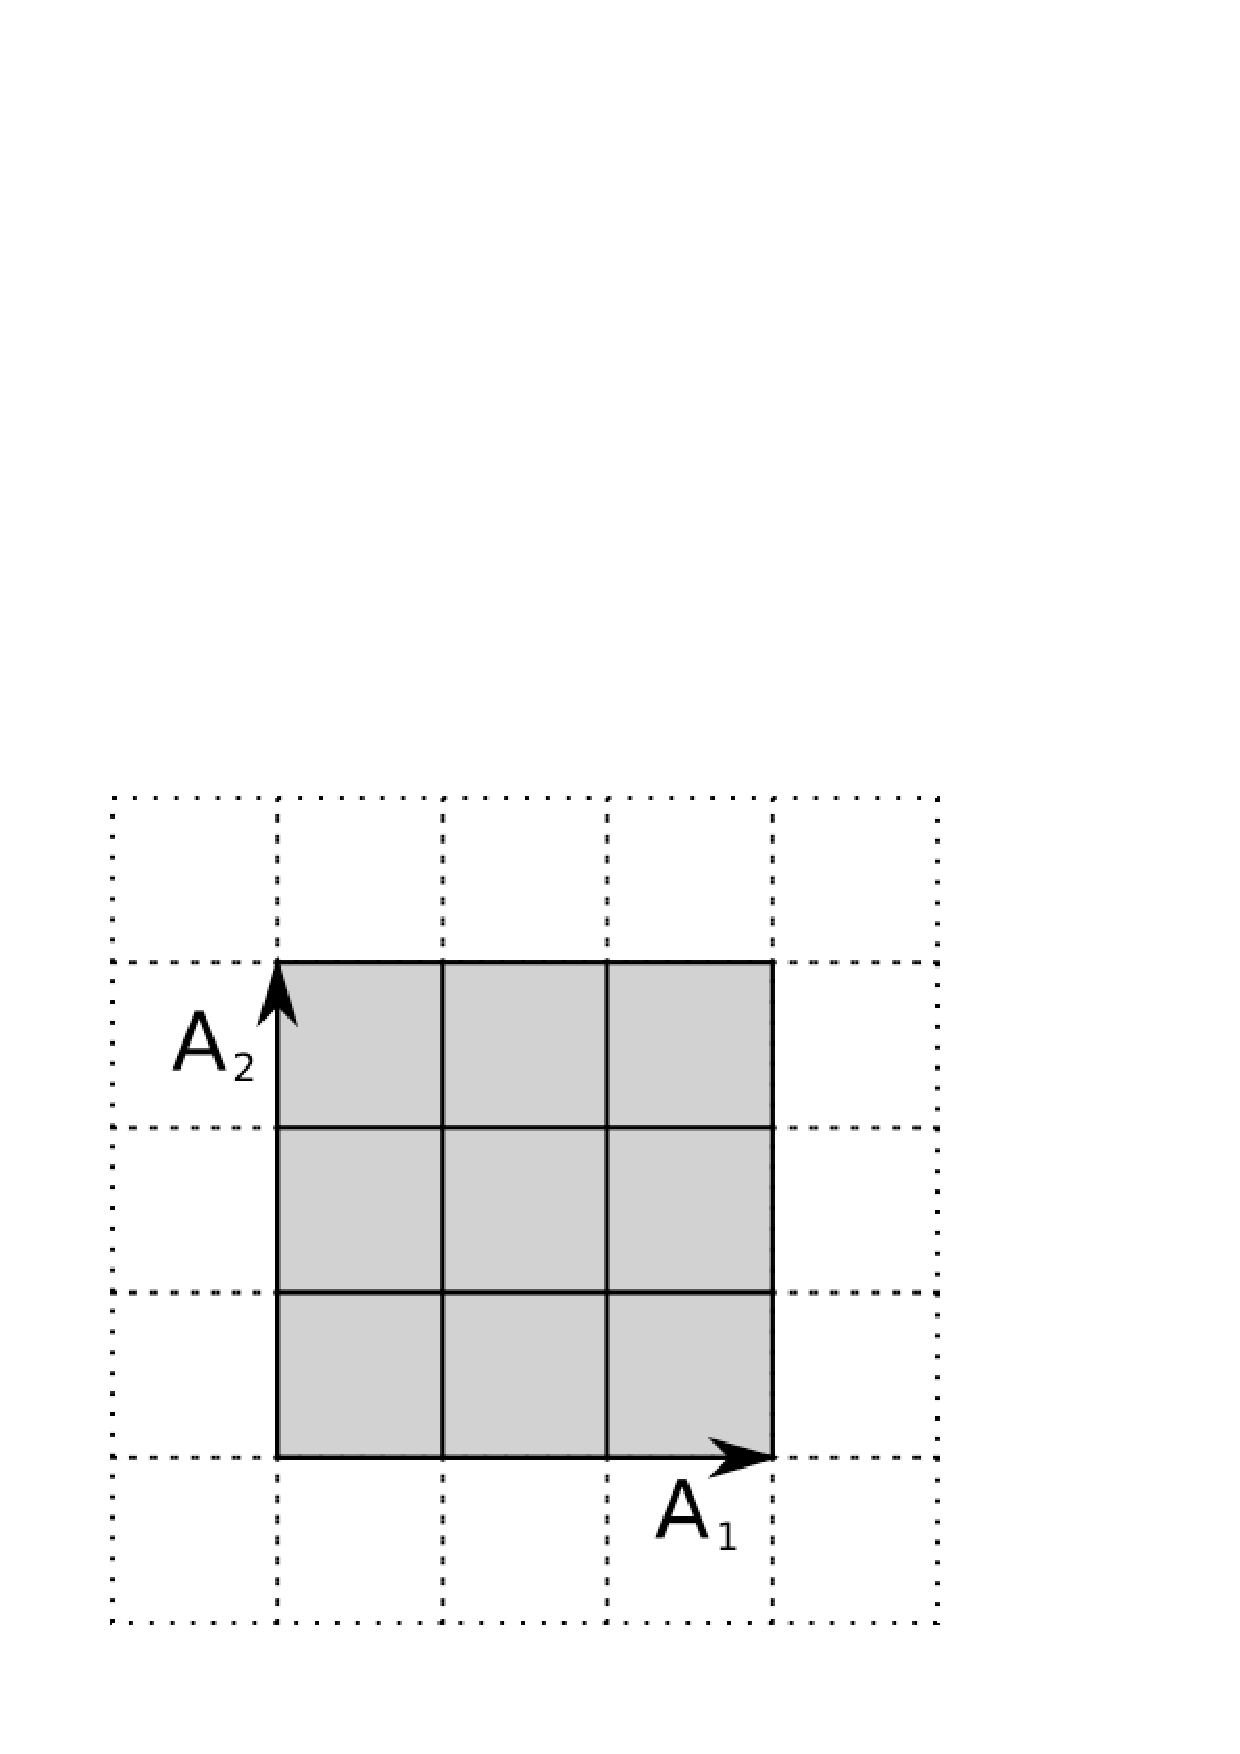
\includegraphics{figures/3x3.pdf}}
\caption{\label{fig:N9} An example of a perfect square packing with density 1: $N=9$.}
\end{figure}

\begin{figure}[H]

\scalebox{.4}{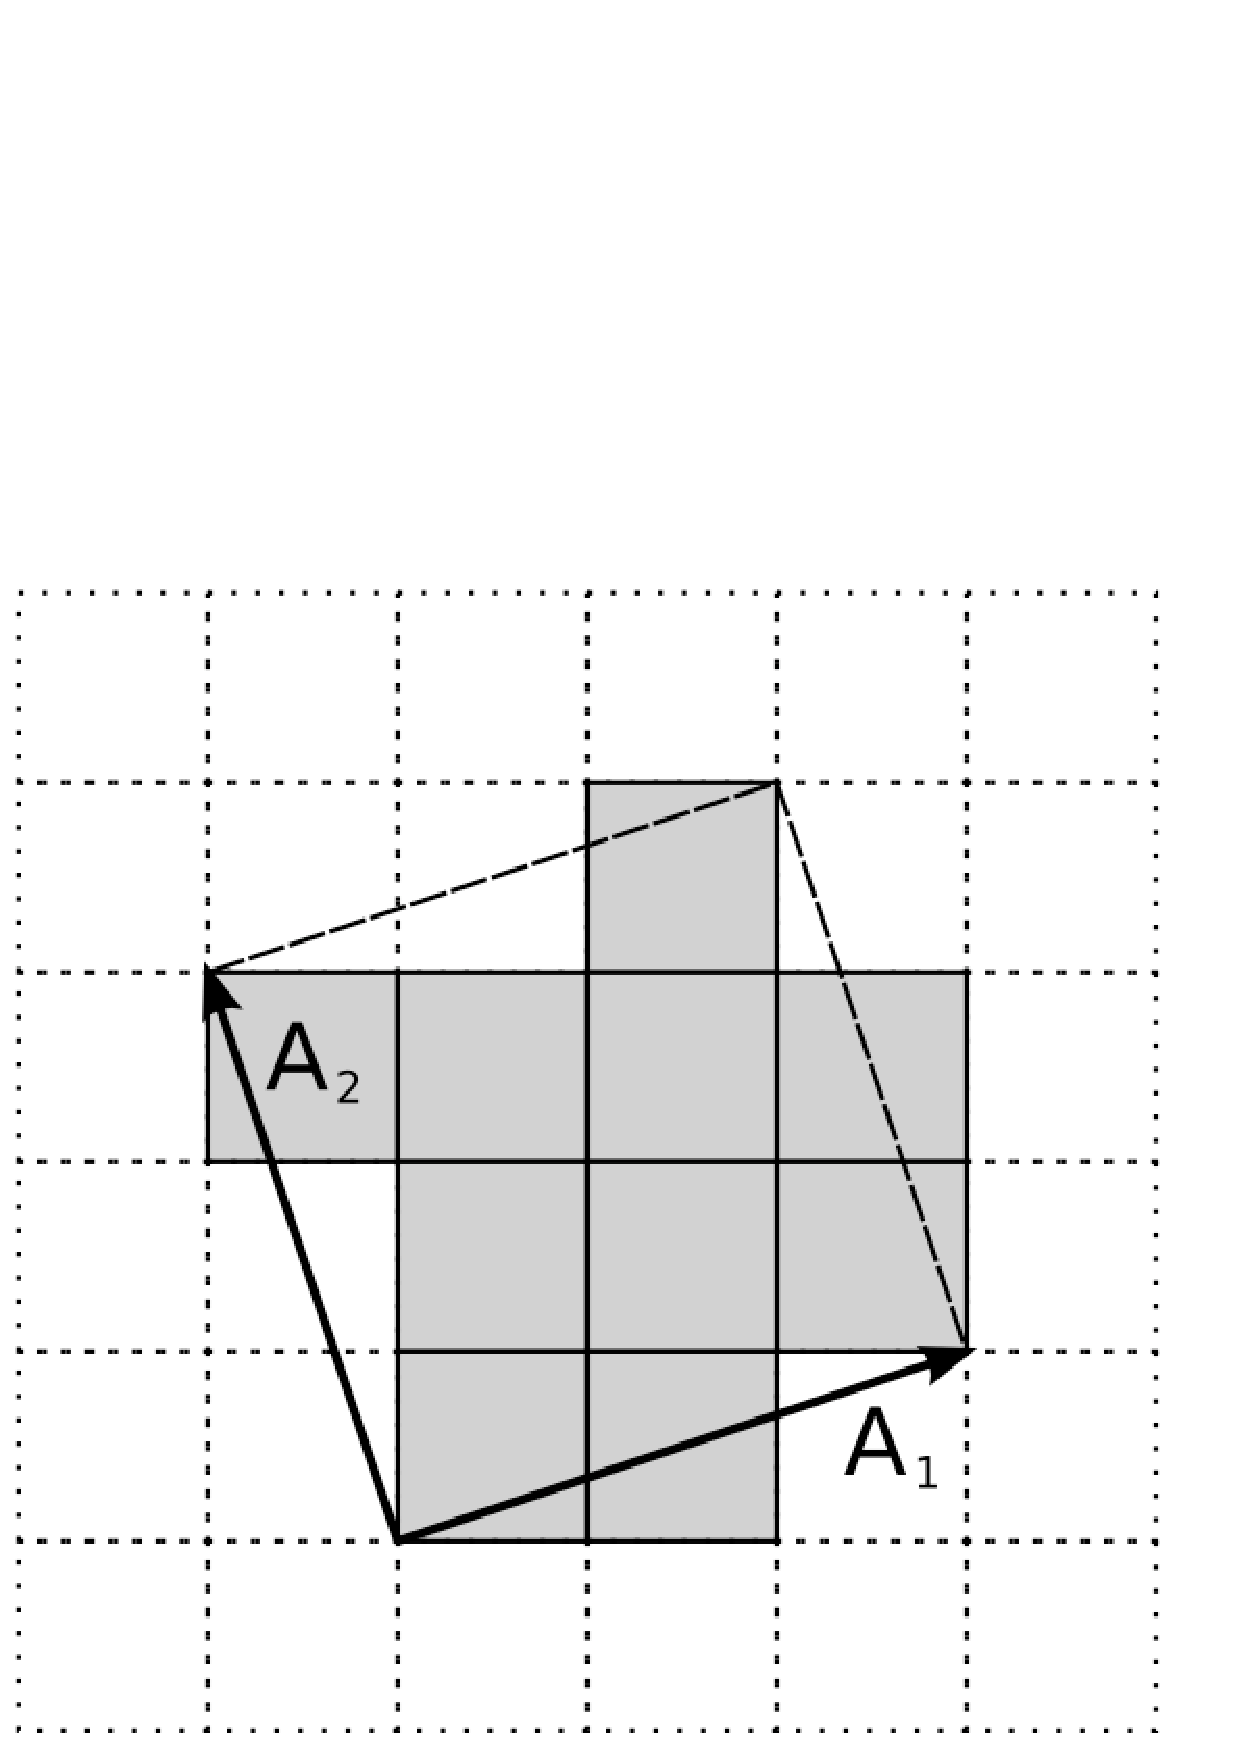
\includegraphics{figures/bravais1.pdf}}
\caption{\label{fig:bravais}An example of a packing for which $N$ is equal to the sum of two squares: $N=10$; all such packings are density $1$.}
\end{figure}

\begin{figure}[H]

\scalebox{.4}{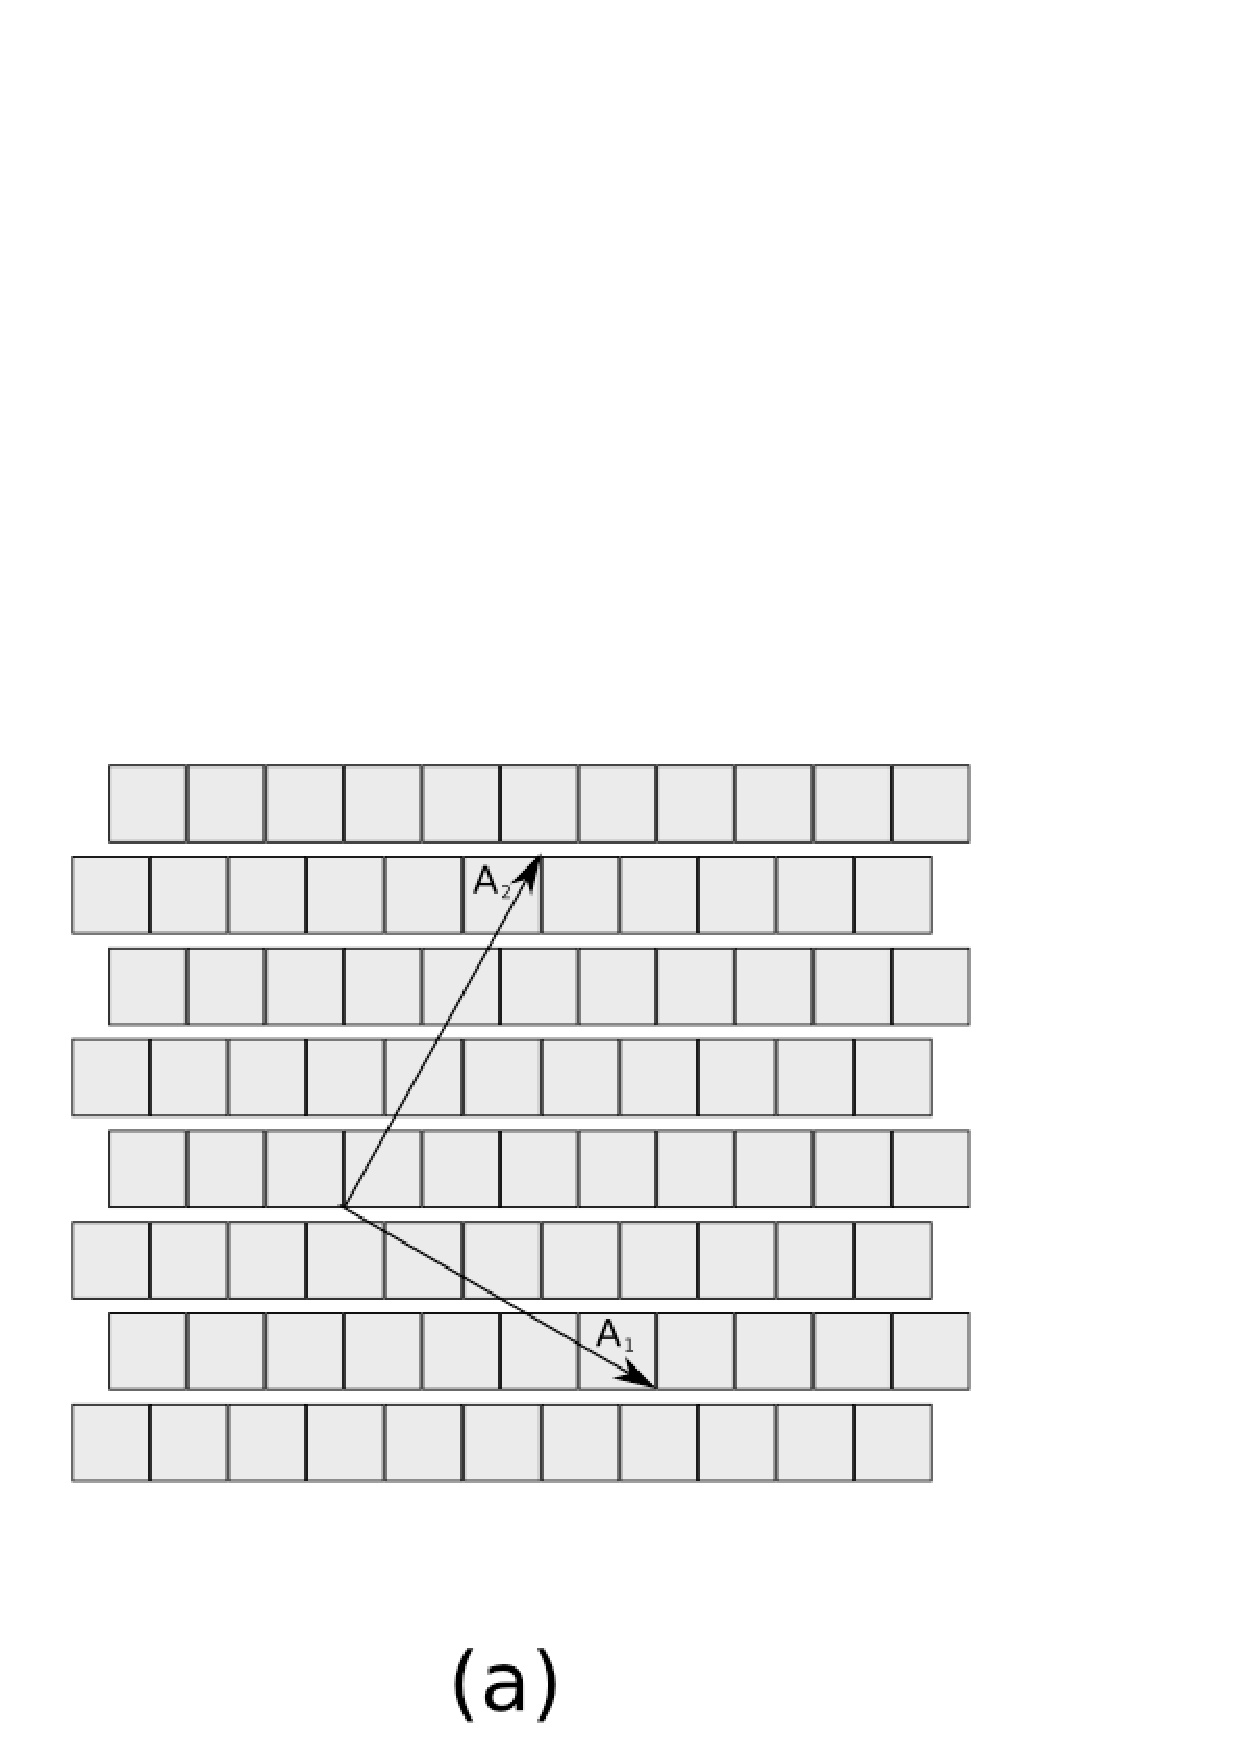
\includegraphics{figures/gappedCombo1.pdf}}
\caption{\label{fig:gb}Schematic (a) of a ``gapped bricklayer'' configuration, with density $\rho = (N-1)/N$. Results of simulated annealing for $N=11$ are shown in (b).}
\end{figure}

\begin{figure}[H]

\scalebox{.45}{\includegraphics{figures/N22.pdf}}
\caption{\label{fig:n22}Simulation results for $N=22$: the conjectured best packing is a ``gapped bricklayer with domino bricks''.}
\end{figure}


\begin{figure}[H]
\scalebox{.25}{\includegraphics{figures/N12.pdf}}
\caption{\label{fig:n12}Simulation results for $N=12$: a lattice of $\frac{1}{2} \times \frac{1}{2}$ holes.}
\end{figure}

\begin{figure}[H]
\scalebox{.35}{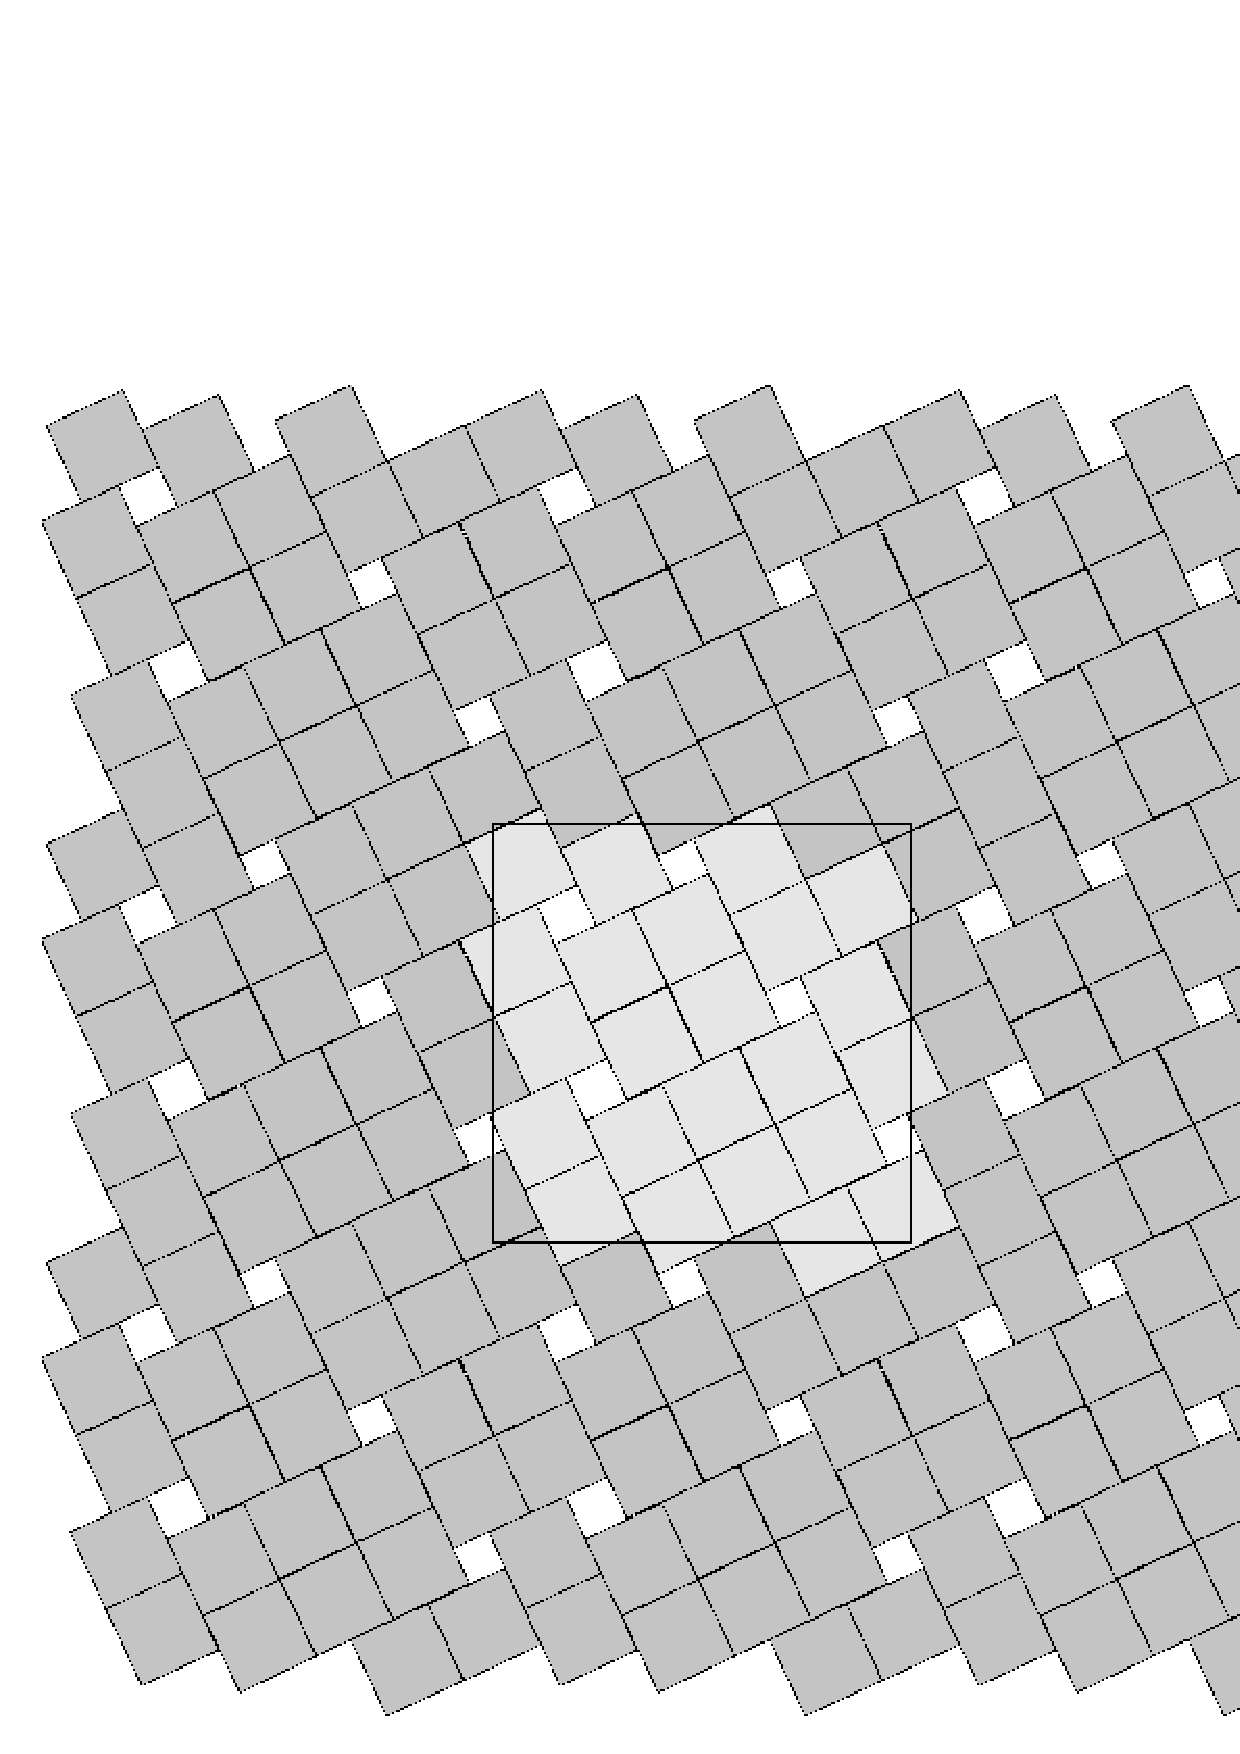
\includegraphics{figures/N23.pdf}}
\caption{\label{fig:n23}Simulation results for $N=23$: a lattice of $\frac{1}{2} \times \frac{1}{2}$ holes.}
\end{figure}

\begin{figure}[H]
\scalebox{.3}{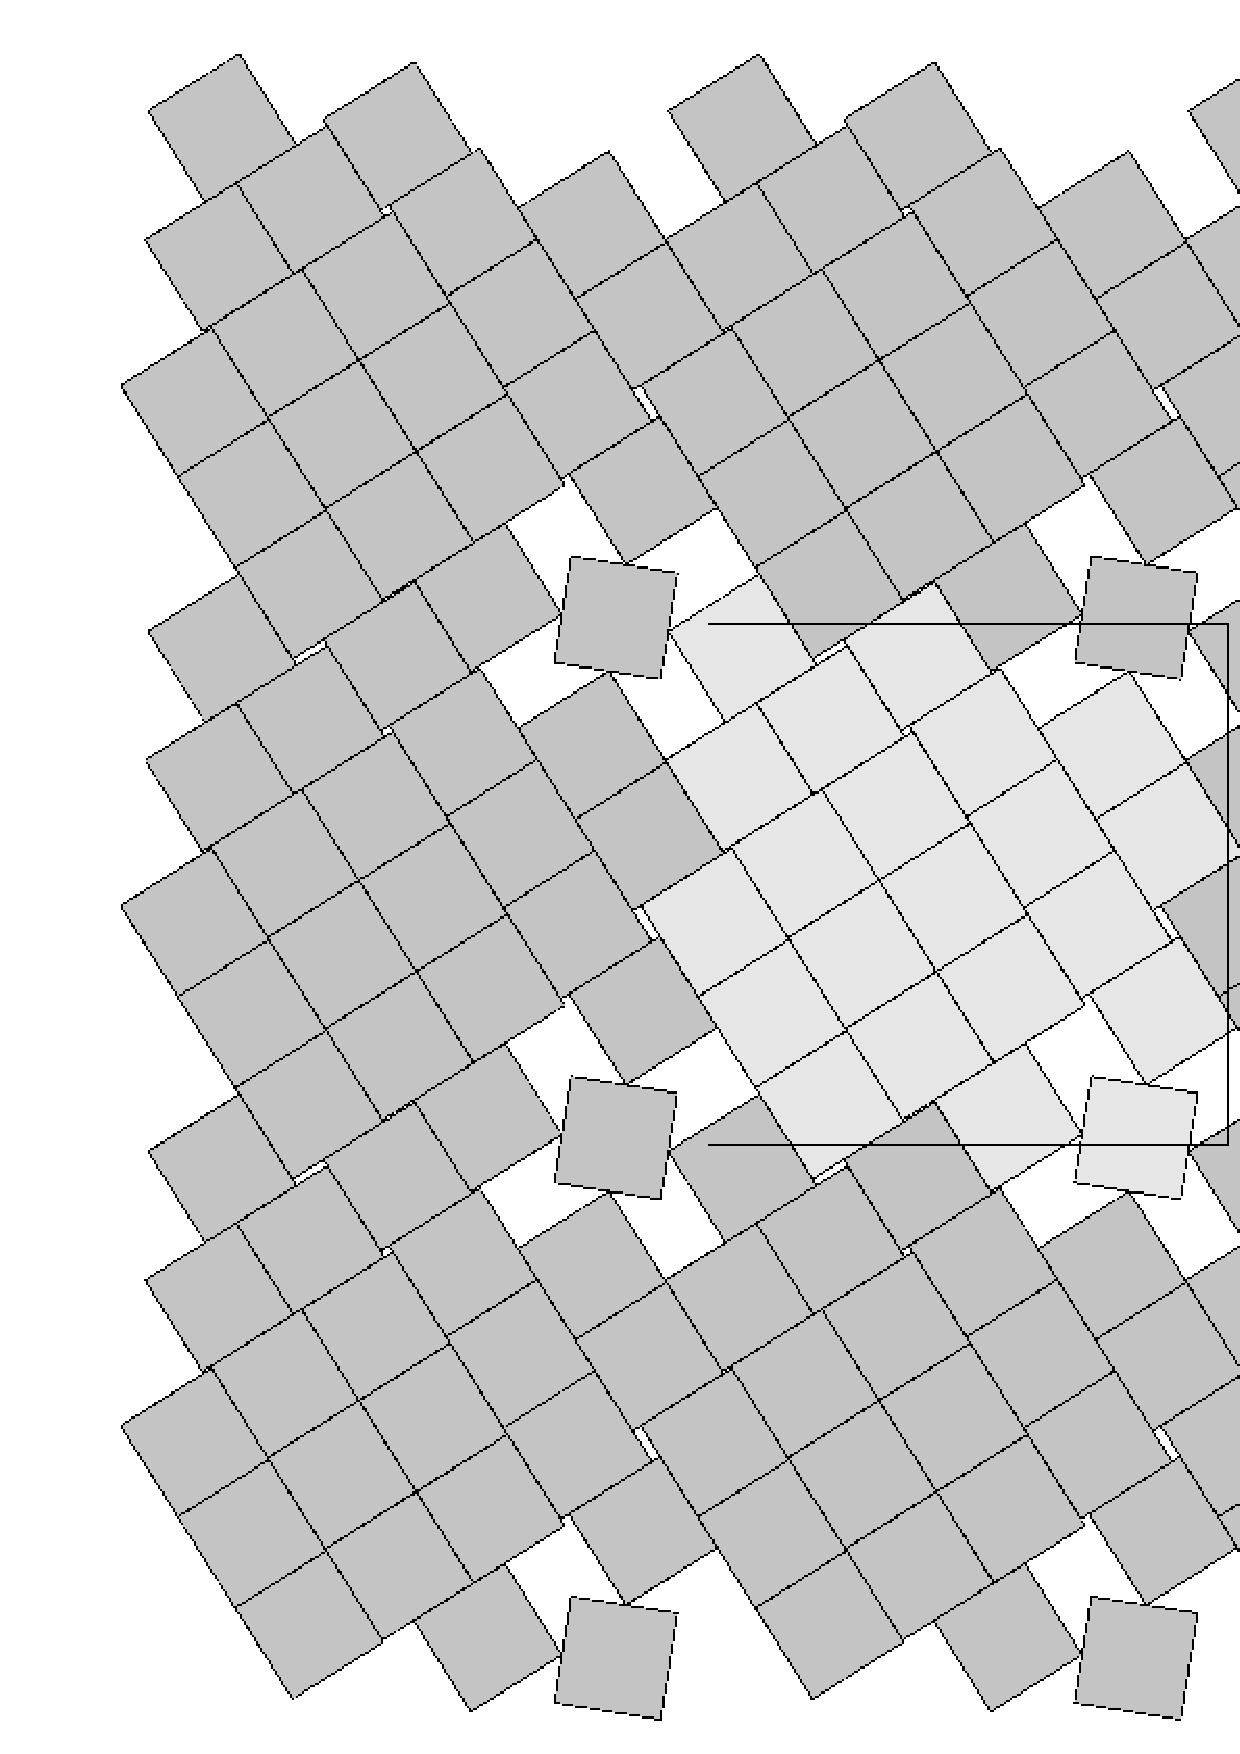
\includegraphics{figures/N21.pdf}}
\caption{\label{fig:n21}Simulation results for $N=21$: a lattice of skew squares embedded in a square lattice.  The $5$-square pattern (which includes a skew square in its center) is the proved best packing of 5 squares in a square \cite{Friedman2002}. Note that the simulation results have not yet converged to the conjectured best packing configuration.}
\end{figure}

\begin{figure}[H]
\scalebox{.3}{\includegraphics{figures/alignedBlocks.pdf}}
\caption{\label{fig:aligned}}
\end{figure}

\begin{figure}[H]
\scalebox{.3}{\includegraphics{figures/pythagoras.pdf}}
\caption{\label{fig:pythagoras}}
\end{figure}


\begin{figure}[H]
\scalebox{.4}{\includegraphics{figures/Bezout1.pdf}}
\caption{\label{fig:Bezout}}
\end{figure}

  
\bibliographystyle{apsrev}
\bibliography{squares}

\begin{acknowledgements}
We would like to thank James Hanna and Narayanan Menon for useful discussions of some of the issues addressed in this paper.  J.M. gratefully acknowledges support from a National Science Foundation grant DMR-0907235. C.S. gratefully acknowledges support National Science Foundatoin grant DMR-0846582. D.B. is grateful for use of the Hoffman2 computing cluster at UCLA.
\end{acknowledgements}

\end{document}

 
